\chapter{Evaluation Method} % Main chapter title

\label{Chapter5} % Change X to a consecutive number; for referencing this chapter elsewhere, use \ref{ChapterX}

\section{Data Collection}
To do evaluation, we first gather baseline performance data from SMAUG. The DLA architecture we
choose to simulate is the DLA provided by SMAUG: a NVDLA-inspired convolution engine with
32-way multiply-accumulate (MACC) arrays and three SPMs. We configure and test our DLA with
a constant three SPM configuration with varying sizes. We test on 32Kb, 64Kb, 128Kb, 256Kb,
512Kb, 1024Kb, 2048Kb size variations. For each configuration, the following models were
evaluated on: VGG, Lenet5, Minerva, Resnet, Cifar-CNN, Elu, Large-Elu, and LSTM. The baseline
strategy is ran in conjunction with the intra-node optimizations SMAUG applies already such
as tile reordering, tile chunk size tuning, loop unrolling, and pipelined DMA transfers. Thus,
the metrics gathered using our pinning strategy are in effect on top of any gains made by
intra-node optimizations.

The metrics we consider most important to measure are the speedup and total
data transfer reduction. We show total speedup to see how much of a practical
performance gain we can obtain using an ideal pining strategy for all workloads.
We are interested in the total data transfer reduction since the speedup is 
dependant on how memory bound a particular DNN model's workload is based on the type
of operations it uses and its graph connections. Thus, based on the memory boundness
of a model, we can estimate how close we reach the theoretical upper bound, i.e
no DMA transfers at all, of speedup we achieve with our model.

The baseline performance for a non-optimized SPM managmenet strategy is
collected by running the simulation in SMAUG and reading the total accelerator
and DMA cycles used to run inference. The DMA cycles are included in the total
accelerator cycles, so we can calculate the fraction of inference time spent on
DMA transfers, hence get a metric of how memory bound a particular DNN model
is.
\[
    Memory\ Boundness = (total\ accelerator\ cycles - DMA\ cycles) / total\ accelerator\ cycles
\]

The upper bound of potential speedup from memory transfer savings is given by

\[
    Potential\ Speedup = 1/(1 - Memory\ Boundness)
\]

Such a speed up is only possible when there are no memory transfers at all and all
inputs and weights are preloaded from the beginning.

%For each of the models, we gather the total accelerator cycles and DMA cycles
%used to perform an inference run.
%
The number of data transfers from the each SPM management strategy is obtained
by summing over the number of transitions in the mapping matrix. We compare the
two sums between the non-optimized and optimized strategies to estimate a speed
up and DMA transfers saved factor. We call the fraction of data transfers saved
over the total data transfers of the unoptimized strategy the reduction factor.

\[
	Total\ Data\ Transfers = \sum_n \sum_k \sum_m |x[n][k][m+1] - x[n][k][m]|\\
\]
\[
	Data\ Transfers\ Saved = Total\ Data\ Transfers\ UnOptimized - Total\ Data\ Transfers\ Optimzed
\]
\[
	Reduction\ Factor = Data\ Transfers\ Saved / Total\ Data\ Transfers\ UnOptimized
\]

With the number of total data transfers saved, we can estimate a potential speedup
based on the memory boundless of a particular model. This is done by estimating what
the new total cycles would be by subtracting the saved DMA cycles based on the reduction
factor. The formula to obtain the speedup is as follows:
\[
	Speedup = (total\ accelerator\ cycles / (total\ accelerator\ cycles - DMA\ Cycles *
	Reduction\ Factor))
\]

\section{Limiting Factors}
A key limiting factor to our model and how we evaluate our cost savings is how
we model tiling. Tiling is invisible from an inter-graph level. As a
consequence, for inputs and outputs that are required to be tiled due to the
tensor size being larger than any scratchpad on the DLA, it would break the ILP
constraint that tensors must be at most the size of the scratchpad.  To
properly take tiling into account, a graph can be reconfigured such that a
single operation broken up into many operations
sequentially scheduled next to each other as shown in figure. %TODO FIGURE%
This will show the effects of the extra data transfers necessary such that the 
ILP model can account for them. We leave the extension to reconfigure graphs
to incorporate tiling for future work. Instead, for our purposes to get
estimate upper bound achievable performance metrics, we resize all tensors
that must be tiled to the scratchpad size. This way we force tensors that
are not immediately reused to be evicted from the scratchpad. Further, because
the baseline model also does not take into account tiling, the speedup and 
transfer costs may be consistent on a relative basis for a graph reconstructed
to account for tiling.


\begin{figure}[th]
\centering
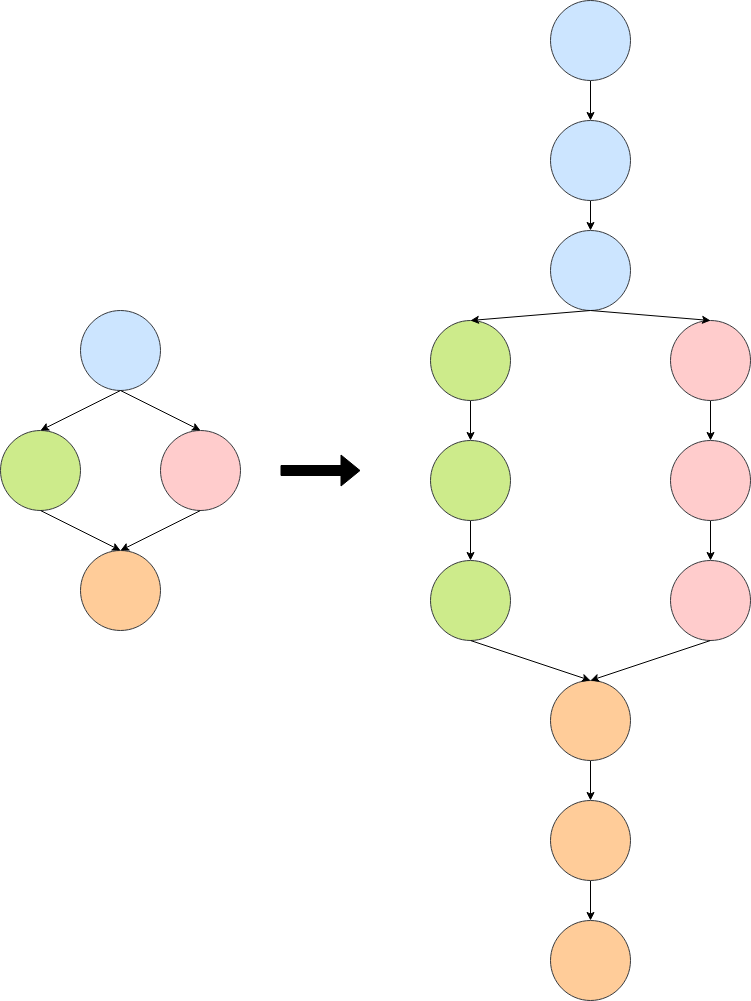
\includegraphics[scale=0.5]{Figures/tiling_regraph.png}
\decoRule
\caption[Saved]{A graph reconverted to account for tiling}
\label{fig:Saved}
\end{figure}

